% ----------------------------------------------------------------
% Article Class (This is a LaTeX2e document)  ********************
% ----------------------------------------------------------------
\documentclass[12pt]{article}
\usepackage[english]{babel}
\usepackage{amsmath,amsthm}
\usepackage{amsfonts}
\usepackage{commath}
\usepackage{fancyhdr}
\usepackage{float}
\usepackage[a4paper,margin=2.0cm,footskip=.5cm]{geometry}
\usepackage[pdftex]{graphicx}
\usepackage[colorlinks=true,
	linkcolor=MidnightBlue,
	urlcolor=BlueViolet,
	citecolor=MyGreen]{hyperref}
\usepackage{listings}
\usepackage[detect-weight,detect-mode]{siunitx}
\usepackage[dvipsnames]{xcolor}

\lstset{
	%        backgroundcolor=\color{lightgray},
	basicstyle=\footnotesize\ttfamily, % Standardschrift
	breaklines=true,            % Zeilen werden Umgebrochen
	extendedchars=true,         %
	frame=b,
	frame=none,
	framexleftmargin=17pt,
	framexrightmargin=5pt,
	framexbottommargin=4pt,
	framextopmargin=0pt,
	keywordstyle=\color{blue},
	%        keywordstyle=[1]\textbf,    % Stil der Keywords
	%        keywordstyle=[2]\textbf,    %
	%        keywordstyle=[3]\textbf,    %
	%        keywordstyle=[4]\textbf,   \sqrt{\sqrt{}} %
	%		 numbers=left,               % Ort der Zeilennummern
	language=matlab,
	numberstyle=\tiny,          % Stil der Zeilennummern
	numbersep=5pt,              % Abstand der Nummern zum Text
    upquote=true,
	stringstyle=\color{BrickRed}\ttfamily, % Farbe der String
    commentstyle=\color{Green},
    % commentstyle=\color{MyGreen},
	showspaces=false,           % Leerzeichen anzeigen ?
	showstringspaces=false      % Leerzeichen in Strings anzeigen ?
	showtabs=false,             % Tabs anzeigen ?
	%		 stepnumber=2,               % Abstand zwischen den Zeilennummern
	tabsize=2,                  % Groesse von Tabs
	%		texcl=true,
	xleftmargin=17pt,
}

\lstloadlanguages{python}
\pagestyle{fancy}
\fancyhf{}
\rhead{Assignment 4: IIR-Filters}
\fancyfoot[C]{\thepage}
\fancyhead[L]{\setlength{\unitlength}{1mm}
    \begin{picture}(0,0)
        \put(0, -1){
\includegraphics[width=1cm]{Resources/img/bsa.png} BSA, WS 24/25}
\end{picture}} 

% ----------------------------------------------------------------
\begin{document}

\section*{Assignment 4: IIR filters}

This assignment makes use of a number of new packages:

\begin{description}
    % \item[mat4py] For more complex \emph{Matlab}-files
    \item[pydicom] For reading in DICOM images
    \item[scikit-image] For image processing
\end{description}

You probably have to manually install two of these packages. To do so, open a
\emph{command terminal}, and enter the following commands:
\begin{lstlisting}
    pip import mat4py
    pip import pydicom
\end{lstlisting}


\section{Finding Filter Coefficients}

\begin{itemize}
    \item Implement the filter for the transfer function \\
        $y(n) = 0.7548 * x(n) - 0.7548 * x(n-1) + 0.5095 * y(n-1)$
    \item Apply it to an impulse input, and to a step input.
    \item What type of function is implemented here?
\end{itemize}


\section{Compare FIR and IIR Filter}

\begin{itemize}
    \item Import ECG Data \lstinline{ecg_hfn.mat}, using
        \lstinline{scipy.io.loadmat}. The data file in
        \emph{Matlab}-format contains a single vector with the name
        \texttt{ecg\_hfn}, and has been recorded with a sample rate of
        \SI{1000}{Hz}.

    \item Calculate coefficients for a window based FIR filter using
        \lstinline{scipy.signal.firwin} to remove high frequency noise.

    \item Calculate coefficients for a butterworth  IIR filter using
        \lstinline{scipy.signal.butter} to remove high frequency noise.

    \item Adjust the filter order for both filters, and display them on the
        command line.
        
    \item Superpose all three signals in a plot.
\end{itemize}

\section{Pulse-Oximetry}

You are a member of a team that wants to investigate the potential for a simple,
non-invasive measure of respiratory effort based on the pulse oximeter signal -
the photoplethysmogram or ‘pleth’. (See also
\href{run:Addison2017.pdf}{Addison2017.pdf}.)

\begin{itemize}
    \item The data in \lstinline{pleth.pickle} contain a dictionary with a
        plethysmography recording from a patient monitor.

    \item Read in the data, using \lstinline{pickle}. For this the Python-command
        \texttt{with} can be very  helpful (you may want to look up that command
        in the Python documentation!):

    \begin{lstlisting}[language=python]
    # From a pickled dictionary:
    in_file = 'data/pleth.pickle'
    with open(in_file, 'rb') as fh:
        data = pickle.load(fh)
        rate = data['rate']
        pleth = data['pleth']
    \end{lstlisting}



    \item Use a low-pass filter to extract the signal components related to
        breathing.

    \item Use a high-pass filter for the heartbeat components. (Note: for
    patient monitoring, the typical frequency range is \SI{0.67}{Hz} $\sim$ 
    \SI{40}{Hz}.)

    \item Plot both signals in separate subplots. The result should look
        approximately as shown below.

    \item Can you also apply a bandpass-filter?
\begin{figure}[H]
    \centering
    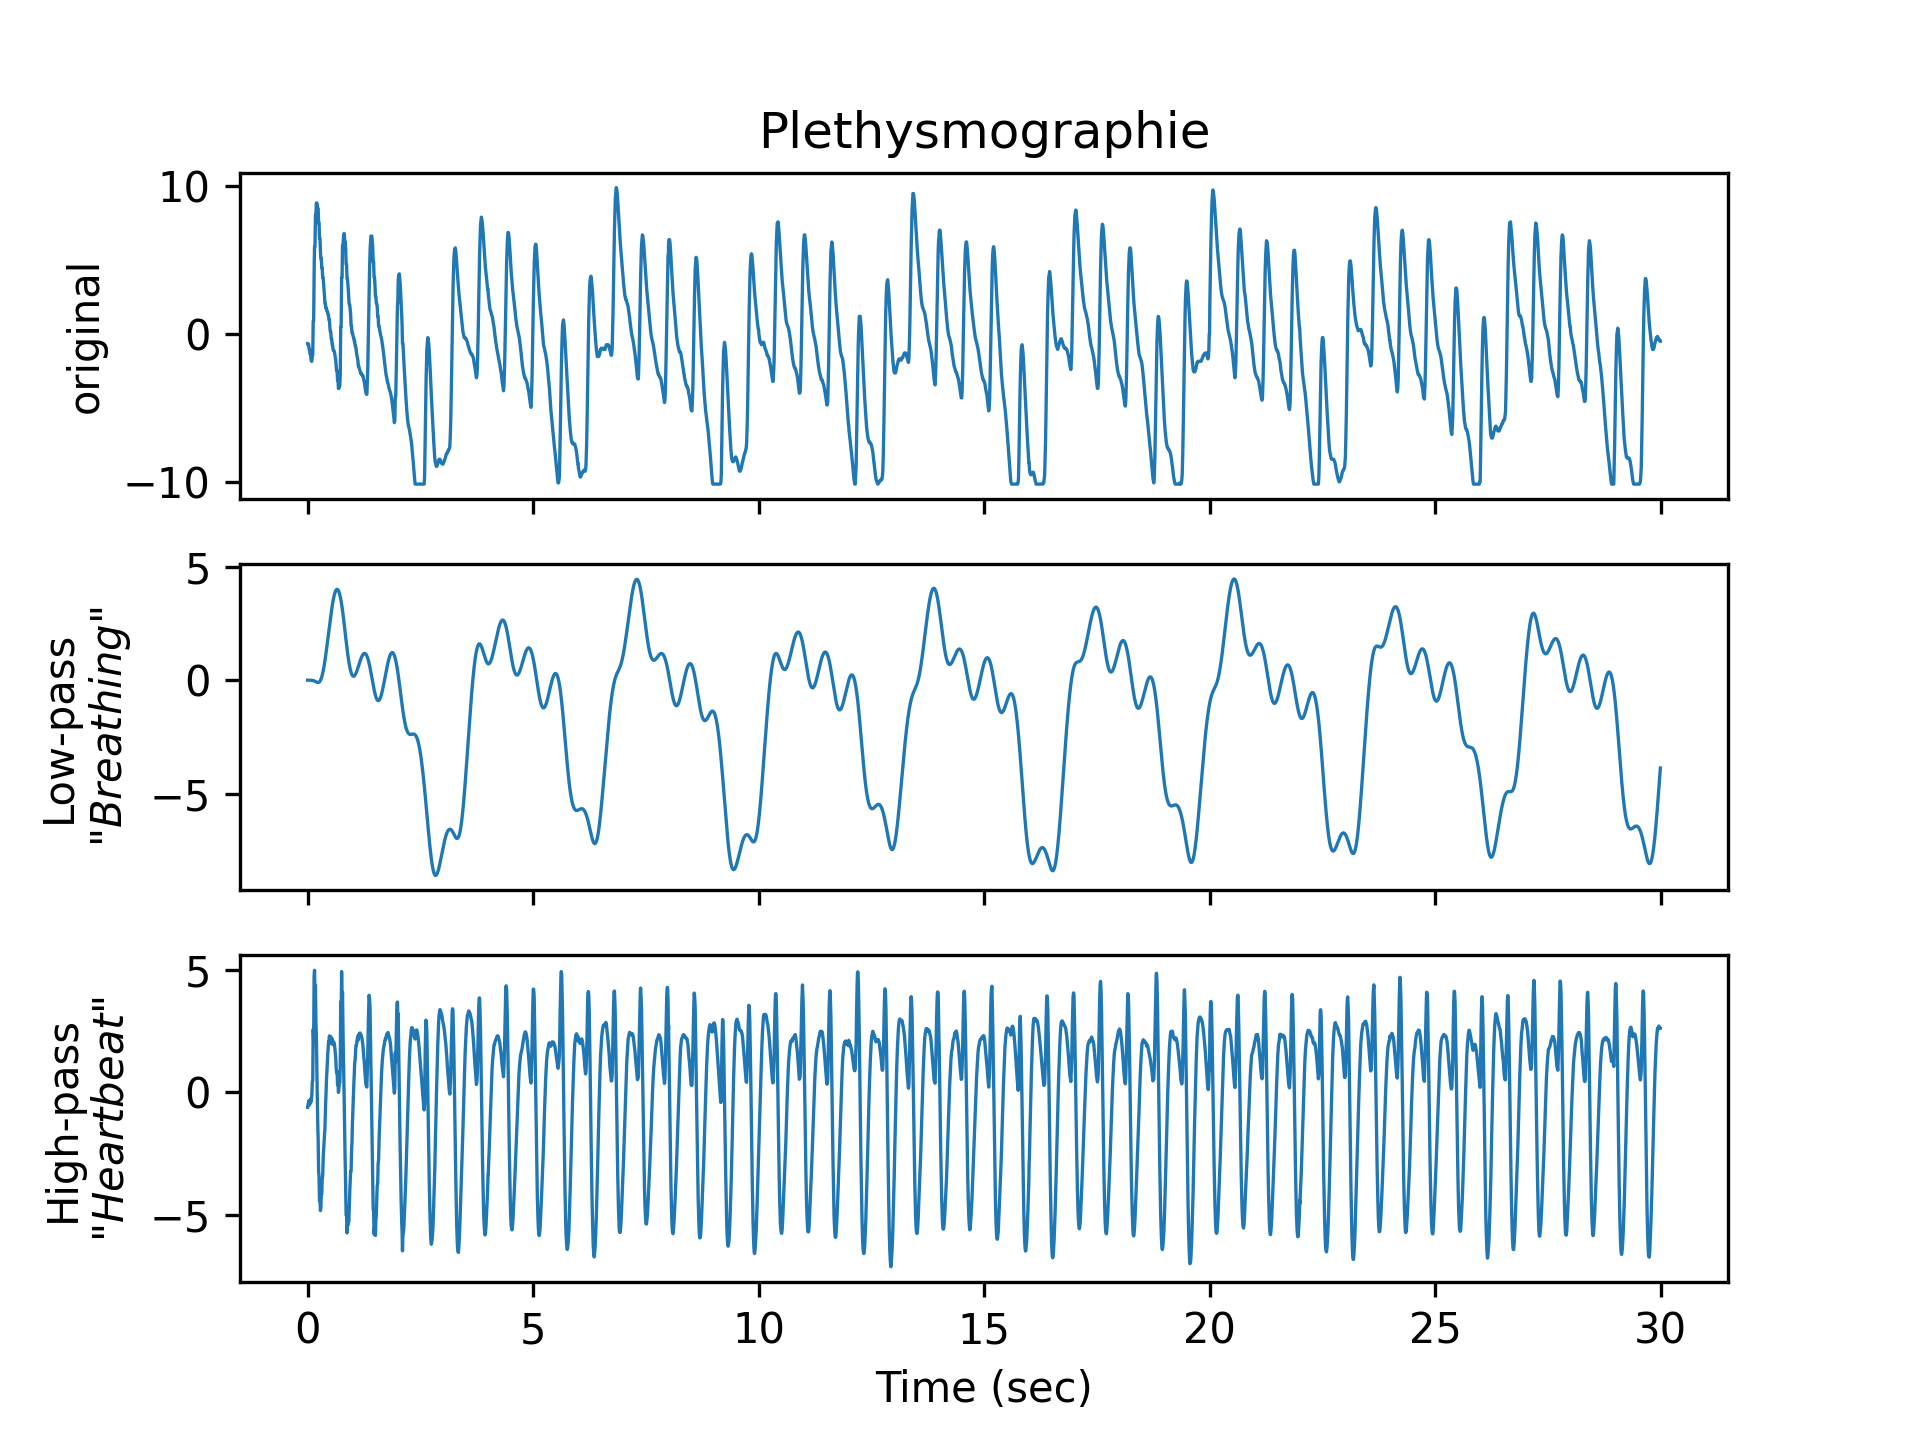
\includegraphics[width=0.75\linewidth]{Resources/img/pleth.png}
\end{figure}

\end{itemize}

\section{Image Processing - Line Detection}%

A good (introduction) to image processing in Python is given in Hands-on Signal Analysis with Python, pp. 96-102

\begin{itemize}

    \item Read in the DICOM-data from \lstinline{MR_MONO2-16-knee}, using
        \lstinline{pydicom.read_file}. This gives you the image data in the
        property \lstinline{pixel_array}.

    \item Display the data.

    \item Find edges using \lstinline{skimage.filters.sobel}, and display them
        in a second plot (in the same figure).

\end{itemize}

\end{document}
% ----------------------------------------------------------------
